\chapter{Raíces de ecuaciones}

\begin{chapquote}{Lozano, 2024}
    ``No se preocupen si no lo entienden, yo tampoco.''
\end{chapquote}

\section{Antecedentes matemáticos}

En general, existen dos tipos de funciones matemáticas:

\begin{definition}[Función algebraica]
    En el caso de una variable, se dice que una función \(f(x)\) es
    algebraica si se expresa de la siguiente manera:

    \[
        f_n y^n + f_{n-1} y^{n-1} + ... + f_1 y + f_0 = 0
    \]

    Donde cada \(f_i (i = 0, 1, ..., n)\) es un polinomio de la forma:

    \[
        f_i = a_{in} X^i + a_{i(n-1)} x^{i-1} + ... + a_{i1} x + a_{i0}
    \]
\end{definition}

\begin{definition}[Función trascendental]
    Es aquella que no es algebraica.
\end{definition}

\begin{eg}
    Las funciones trigonométricas, exponenciales, logarítmicas, las de
    Bessel, Jacobi, Mittag Leffler, entre muchas otras, son trascendentes.
    Por ejemplo, el logaritmo natural se puede definir así:

    \[
        \boxed{\ln(x) = \int_1^x \frac{d \tau}{\tau}, x > 0}
    \]

\end{eg}

Solucionar ecuaciones algebraicas o trascendentes implica el uso de dos tipos
de métodos numéricos: los métodos cerrados y los métodos abiertos. Los primeros
utilizan dos valores que encierran a la raíz entre dos valores, mientras que
los segundos sólo acotan con un valor.

\section{Métodos cerrados}

Este tipo de métodos aprovecha el cambio de signo que se presenta cuando una
función pasa a través del eje de las abscisas para detectar una raíz. Se les
conoce por ese nombre porque necesitan un intervalo cerrado que contenga a la
raíz. Un método cerrado muy sencillo, y el primero que será revisado en esta
sección, es el \emph{método de bisección}.

\subsection{Método de bisección}

En general, si $f(x)$ es una función real y continua en el intervalo $[x_l,
x_u]$ \footnote{Aquí, $l$ y $u$ vienen de la palabras inglesas \textit{lower} y
\textit{upper}.} y además $f(x_l)$ y $f(x_u)$ tienen signos opuestos,
\textit{i.e.} $f(x_l) \cdot f(xu) < 0$, se sabe que \emph{existe al menos una
raíz entre $x_l$ y $x_u$}.

El método consiste en dividir el intervalo original a la mitad (hacer una
bisección) y descartar aquella mitad donde no haya raíces. El proceso se repite
tantas veces como sea necesario hasta que el intervalo sea, en términos
prácticos, un sólo punto: la raíz buscada. Este método para encontrar raíces se
parece al algoritmo \textit{binary search} para encontrar un valor dado entre
una lista de valores.

\subsubsection{Algoritmo para el método de bisección}

\begin{enumerate}
    
    \item Elija el intervalo que encierra la raíz, es decir, $[x_l, x_u]$.
        Verifique que $f(x_l) \cdot f(x_u) < 0$.

    \item Obtenga la aproximación de la raíz con $x_r \approx \frac{x_l +
        x_u}{2}$

    \item Para determinar el nuevo sub-intervalo, revise los siguientes casos:
        \begin{itemize}
            \item Si $f(x_l) \cdot f(x_r) < 0$, entonces la raíz debe
                encontrarse en el intervalo $[x_l, x_r]$. El algoritmo se
                seguirá ejecutando de manera recursiva.

            \item Si $f(x_l) \cdot f(x_r) > 0$, entonces la raíz debe
                encontrarse en el intervalo $[x_r, x_u]$. El algoritmo se
                seguirá ejecutando de manera recursiva.

            \item Si $f(x_l) \cdot f(x_r) = 0$, o \(\varepsilon_a <
                \varepsilon_s\), entonces $x_r$ es la raíz buscada. Aquí,
                $\varepsilon_a$ es el \emph{error relativo aproximado} y
                $\varepsilon_s$ es la \emph{tolerancia} (\textit{sufferance})
                prefijada.

        \end{itemize}
\end{enumerate}

Pocas veces se conoce \textit{a priori} el valor de la raíz real. Por ello, se
debe definir una aproximación mediante el error relativo aproximado:

\[
    \varepsilon_a = \left| \frac{x_i - x_{i-1}}{x_i} \right| \times 100\%
\]

Una fórmula comúnmente usada para la elegir una tolerancia en cálculos numéricos
donde se quiere garantizar un número $n$ de cifras significativas es la
siguiente:

\[
    \varepsilon_s = 0.5 \times 10^{2-n} \%
\]

\begin{ex}

    Encuentre la raíz de la ecuación \ref{primer-problema}:

    \[
        x^2 - 4 - sin(x) = 0
    \]

    \begin{solution}
        Tomando $f(x) = x^2 - 4 - sin(x)$, uno puede utilizar un
        lenguaje de programación para implementar el algoritmo ya
        descrito.

        \lstinputlisting[language=Fortran, caption=Implementación del
        método de bisección en Fortran.,
        label={lst:bisect-fortran}]{./programas/metodo-biseccion/biseccion.f90}

        \lstinputlisting[language=Go, caption=Implementación del
        método de bisección en Go.,
        label={lst:bisect-go}]{./programas/metodo-biseccion/biseccion.go}
    \end{solution}
    
\end{ex}

\subsection{Método de la falsa posición}

Como se vio anteriormente, el método de bisección es bastante útil para hallar
raíces de ecuaciones el cual únicamente usa fuerza bruta. \emph{No obstante, su
tiempo de cómputo en comparación de otros métodos es alto}. Una alternativa a
tal método es el de la \emph{falsa posición}, el cual tiene la siguiente
ecuación recursiva:

\[
    \boxed{x_r = x_u - \frac{f(x_u) (x_l-x_u)}{f(x_l) - f(x_u)}}
\]

\subsubsection{Algoritmo para el método de la falsa posición}

\begin{enumerate}
    
    \item Elija el intervalo que encierra la raíz, es decir, $[x_l, x_u]$.
        Verifique que $f(x_l) \cdot f(x_u) < 0$.

    \item Obtenga la aproximación de la raíz con
        \[
            x_r \approx x_u - \frac{f(x_u)(x_l-x_u)}{f(x_l) - f(x_u)}
        \]

    \item Para determinar el nuevo sub-intervalo, revise los siguientes casos:
        \begin{itemize}
            \item Si $f(x_l) \cdot f(x_r) < 0$, entonces la raíz debe
                encontrarse en el intervalo $[x_l, x_r]$. El algoritmo se
                seguirá ejecutando de manera recursiva.

            \item Si $f(x_l) \cdot f(x_r) > 0$, entonces la raíz debe
                encontrarse en el intervalo $[x_r, x_u]$. El algoritmo se
                seguirá ejecutando de manera recursiva.

            \item Si $f(x_l) \cdot f(x_r) = 0$, o \(\varepsilon_a <
                \varepsilon_s\), entonces $x_r$ es la raíz buscada.

        \end{itemize}
\end{enumerate}

\begin{ex}
    Resuelva el ejercicio anterior mediante el método de falsa posición
    
    \begin{solution}

        Puede implementarse el algoritmo descrito anteriormente en un
        programa de computadora de la siguiente manera:

        \lstinputlisting[language=Fortran, caption=Implementación del
        método de la falsa posición en Fortran.,
        label={lst:false-fortran}]{./programas/metodo-falsa-posicion/falsa.f90}

        \lstinputlisting[language=Go, caption=Implementación del
        método de la falsa posición en Go.,
        label={lst:false-go}]{./programas/metodo-falsa-posicion/falsa.go}
    \end{solution}
\end{ex}

Observe que el método de la falsa posición converge, por lo general, más rápido
que el método de bisección. Lo anterior se debe a que, dependiendo de la
naturaleza de $f(x)$, en ocasiones se descarta el intervalo más grande.


\section{Métodos abiertos}

Mientras que los métodos cerrados garantizan la convergencia a una raíz, este
tipo de métodos depende sensiblemente de las condiciones iniciales para su
ejecución, pues divergen con facilidad.

\subsection{Método de punto fijo (o función contraída)}

Este es uno de los métodos más simples. Si se quiere encontrar la raíz de una
función $f(x)$ donde se puede despejar alguna $x$, se puede obtener una
relación de recurrencia para calcular las raíces:

\begin{equation}\label{eqn:punto-fijo}
    f(x_0) = 0 \implies \boxed{x = g(x)}
\end{equation}

Si, eligiendo un dominio $D$ donde exista la raíz, se cumple que
\[
    \left| g'(x) \right| < 1 \land x \in D
\]

\noindent puede transformarse \ref{eqn:punto-fijo} en una relación de
recurrencia:

\begin{equation} \label{eqn:recurrencia-punto-fijo}
    \boxed{x_{i+1} = g(x_i)}
\end{equation}

\begin{ex}
    Use el método de iteración de punto fijo para encontrar las raíces de la
    función:
    \[
        e^{-x} - x = 0
    \]

    \begin{solution}

        Puede encontrase el esquema del método de punto fijo de la siguiente
        forma:

        \[
            f(x) = e^{-x} - x = 0 \implies x = e^{-x} = g(x)
        \]

        Teniendo en cuenta la gráfica de la función en la figura
        \ref{fig:ejercicio-punto-fijo}, la raíz es aproximadamente $x_r \approx
        0.6$, por lo que puede verificarse que la derivada tiene magnitud menor
        a uno:

        \[
            \left| g'(x) \right| = \left| -e^{-x} \right| e^{-x} =
            \frac{1}{e^x} < 1\ \forall x \in (0, \infty)
        \]

        \begin{figure}
            \centering
            \begin{tikzpicture}
                \begin{axis}[xmin=0, xmax=1, ymin=-0.5, ymax=1.5, axis lines=middle]
                    \addplot[color=black, domain=0:1]{e^(-x) - x};
                \end{axis}
            \end{tikzpicture}
            \caption{Función $f(x) = e^{-x} - x$}
            \label{fig:ejercicio-punto-fijo}
        \end{figure}

        Como la condición se satisface, puede escribirse la siguiente ecuación
        de recurrencia basándose en \ref{eqn:recurrencia-punto-fijo}:

        \[
            x_{i+1} = e^{-x_i}
        \]

        Si se toma una $x_0 = 1$ y se empiezan a obtener resultados de
        manera iterativa, $x \rightarrow 0.5671432904$

        % importar tabla
    \end{solution}
\end{ex}

El método tiene este nombre debido a su interpretación geométrica. El valor
inicial $x_0 = 1$, con una vertical toca a $g(x)$, después una horizontal toca a
la función identidad nuevamente. El proceso se repite de manera que se forma una
espiral de donde surge el nombre ``función contraída''

\begin{ex}
    La siguiente ecuación puede resolverse vara valores de $r \in [0,4]$,
    donde $r$ representa la taza de crecimiento poblacional:

    \[
        x - rx(1 - x) = 0
    \]

    \noindent donde, aplicando el método de punto fijo se obtiene la relación
    \[
        x_{n+1} = r x_n (1 - x_n)
    \]

    Esta ecuación es conocida como la \emph{ecuación logística}, que tiene su
    origen en la dinámica de poblaciones, los términos son:
    \begin{align*}
        rx_n &= \text{taza de nacimientos} \\
        (1 - x_n) &= \text{taza de mortandad}
    \end{align*}

    \lstinputlisting[language=Fortran, caption=Código para obtener el
    diagrama de bifurcación mediante el método de punto fijo en Fortran.,
    label={lst:bifurc-fortran}]{./programas/bifurcacion/bifurcacion-logistica.f90}

    \begin{figure}
        \centering
        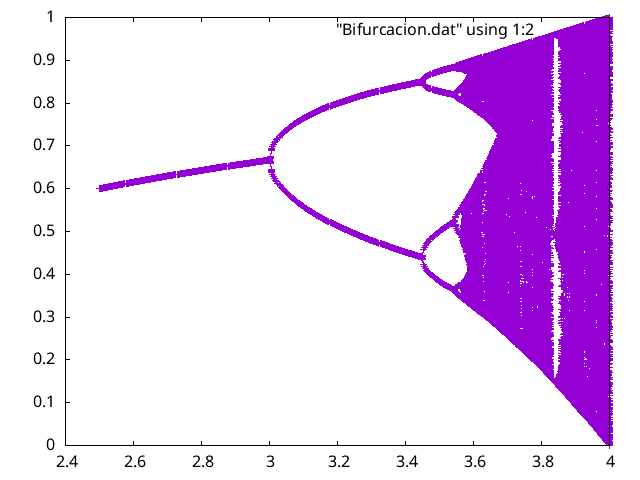
\includegraphics[width=1.0\textwidth]{programas/bifurcacion/bifurcacion.png}
        \caption{Diagrama de bifurcación creado con el programa de
        Fortran y \textit{GNUPlot}.}
    \end{figure}
\end{ex}

\subsection{Método de Newton-Raphson}

El método de Newton-Raphson es popular debido a la facilidad con la que puede
ser implementado, así como por sun velocidad de convergencia cuando se le da un
valor inicial adecuado. El método consiste en el trazo de una recta tangente
desde el punto $(x, f(x))$ e ir acercándose progresivamente a la raíz $x_r$.

El esquema de Newton-Raphson se obtiene a partir de la serie de Taylor truncada
a términos de primer orden,
\[
    f(x) \approx f(x_0) + f'(x_0)(x - x_0)
\]

Si la ecuación
\begin{equation}
    f(x_0) + f'(x_0) (x - x_0) = 0 \label{eqn:newton-aprox}
\end{equation}

\noindent tiene una solución $x = x_r$, puede concluirse que $f(x_r) \approx
0$. Si la función ``se porta bien'', repetir este proceso llevará a valores de
$x_r$ cada vez más cercanos a la raíz verdarera. Despejando $x$ de
\ref{eqn:newton-aprox}, se obtiene la siguiente relación de recurrencia para
obtener aproximaciones de la raíz de $f$ a partir de algún valor inicial
arbitrario $x_0$:

\begin{equation}\label{eqn:newton}
    \boxed{x_{n+1} = x_n - \frac{f(x_n)}{f'(x_n)}}
\end{equation}

\begin{ex}
    Obtenga la raíz de la siguiente ecuación,
    \[
        f(x) = x^3 + x^2 + \ln(x) + 2 \cos(x) = 0
    \]

    \begin{solution}

        Es buena idea obtener la gráfica de la función para poder visualizar
        las intersecciones y elegir un mejor valor inicial.

        \begin{figure}
            \centering
            \begin{tikzpicture}
                \begin{axis}[xmin=0, xmax=1, ymin=-0.5, ymax=2, axis lines=middle]
                    \addplot[color=black, domain=0:1]{x^3 + x^2 + ln(x) + 2 * cos(deg(x))};
                \end{axis}
            \end{tikzpicture}
            \caption{Función $f(x) = x^3 + x^2 + \ln(x) + 2 \cos(x)$}
            \label{fig:ejercicio-newton}
        \end{figure}


        La derivada es 
        \[
            f'(x) = 3x^2 + 2x + \frac{1}{x} - 2 \sin(x)
        \]

        Para encontrar la relación de recurrencia correspondiente de
        Newton-Raphson, puede usarse el siguiente esquema:
        \begin{align*}
            x_{n+1} &= x_n - \frac{f(x_n)}{f'(x_n)} \\
                &= x_n - \frac{x^3 + x^2 + \ln(x) + 2
                \cos(x)}{3x^2 + 2x + \frac{1}{x} - 2 \sin(x)}
        \end{align*}

        La figura \ref{fig:ejercicio-newton}, puede verse que la raíz está
        cerca de $x = 0.15$, puede utilizarse una calculadora para empezar
        estas iteraciones. El resultado es
        \[
            \boxed{x_r \approx 0.1349}
        \]

    \end{solution}

\end{ex}

\begin{ex}
    Encuentre la raíz real del polinomio 
    \[
        18.95x^3 + 5x^2  + 0.33x + 1 = 0
    \]

    \begin{solution}
        Se aplica la fórmula \ref{eqn:newton} para aplicar el método de
        Newton-Raphson
        \begin{align*}
            x_{n+1} &= x_n - \frac{f(x_n)}{f'(x_n)} \\
                &= x_n - \frac{18.95x_n^3 + 5x_n^2 + 0.33x_n +
                1}{3(18.95)x_n^2 + 10x_n + 0.33}
        \end{align*}

        \begin{figure}
            \centering
            \begin{tikzpicture}
                \begin{axis}[xmin=-0.6, xmax=0.2, ymin=-0.2, ymax=1.5, axis lines=middle]
                    \addplot[color=black, domain=-0.5:0.2]{18.95*x^3 + 5*x^2 + 0.33*x + 1};
                \end{axis}
            \end{tikzpicture}
            \caption{Función $f(x) = 18.95\ x^3 + 5\ x^2 + 0.33\ x + 1$}
            \label{fig:ejercicio-newton-2}
        \end{figure}

        Tomando en cuenta la figura \ref{fig:ejercicio-newton-2}, puede
        elegirse como punto inicial a \(x_0 = -0.5 \), y el valor de la raíz
        llega a
        \[
            \boxed{x_{r_1} \approx -0.4677830945}
        \]

        Conociéndose la aproximación para una de las raíces, puede utilizarse
        división sintética para aproximar un polinomio de segundo grado cuyas
        raíces pueden ser calculadas con la fórmula general. A este proceso se
        le conoce como \textit{deflación polinomial}:

        \begin{center}
            \begin{tabular}{ c | c c c c }
                & 18.95 & 5 & 0.33 & 1 \\
                    0.467731 & & -8.8644896 & 1.80774292 & -1 \\
             \hline
                 & 18.95 & -3.8644896 & 2.13774292 & 0
            \end{tabular}
        \end{center}

        Se obtiene el polinomio
        \[
            18.95\ x^2 - 3.8644896\ x + 2.13774292,
        \]

        \noindent cuyas raíces pueden encontrarse con la fórmula general,
        obteniendo las raíces faltantes:
        \begin{align*}
            x_{r_1} & \approx -0.4677831 \\
            x_{r_2} & \approx 0.1019 + 0.32001\ i \\
            x_{r_3} & \approx 0.1019 - 0.32001\ i 
        \end{align*}
    \end{solution}
\end{ex}

\subsection{Método de la secante}

El método de Newton-Raphson que se describió anteriormente y formulado por la
ecuación \ref{eqn:newton} emplea una derivada en el denominador. Si la función
cuyas raíces se quieren encontrar es difícil de derivar, puede que utilizar este
método no sea ideal. En estos casos, se recurre a modificar el método para
sustituir la derivada por un esquema numérico en diferencias finitas centradas
\[
    f'(x_i) \approx \frac{f(x_i) - f(x_{i-1})}{x_i - x_{i-1}}
\]

Sustituyendo esta relación en el esquema normal de Newton-Raphson:

\begin{equation}\label{eqn:secante}
    \boxed{x_{n+1} = x_n - \frac{f(x_n)}{ \left( \frac{f(x_n) - f(x_{n-1})}{x_n - x_{n-1}} \right)}}
\end{equation}

También puede utilizarse la expresión

\begin{equation}\label{eqn:secante-2}
    \boxed{x_{n+1} = x_n - \frac{f(x_n)}{ \left( \frac{f(x_n + h) - f(x_n)}{h} \right)}}
\end{equation}


\begin{ex}
    Encuentre la raíz de la función

    \[
        f(x) = \sin x\ e^{\cos x} * \ln(\cosh x) - 4\ x + x^3
    \]

    \begin{figure}
        \centering
        \begin{tikzpicture}
            \begin{axis}[xmin=-3, xmax=3, ymin=-4, ymax=4, axis lines=middle]
                \addplot[color=black, domain=-3:3]{(sin(deg(x)) * e^(cos(deg(x)) * ln(cosh(x))) - 4 * x + x^3};
            \end{axis}
        \end{tikzpicture}
        \caption{Función $f(x) = \sin x\ e^{\cos x} * \ln(\cosh x) - 4\ x + x^3$}
        \label{fig:ejercicio-secante}
    \end{figure}


\end{ex}

\subsection{Método de Newton multivariable}

Supóngase que se quiere solucionar el siguiente sistema de ecuaciones:

\begin{align*}
    u(x,y) = 0 \\
    v(x,y) = 0
\end{align*}
